% !TeX encoding = UTF-8
% !TeX program = pdflatex
% !TeX spellcheck = en_US
\documentclass[lettersize,journal]{IEEEtran}
\usepackage[scheme=plain,punct=plain]{ctex}
\usepackage{amsmath,amsfonts}
\usepackage{algorithmic}
\usepackage{algorithm}
\usepackage{array}
\usepackage[caption=false,font=normalsize,labelfont=sf,textfont=sf]{subfig}
\usepackage{textcomp}
\usepackage{stfloats}
\usepackage{url}
\usepackage{verbatim}
\usepackage{graphicx}
\usepackage{cite}
\hyphenation{op-tical net-works semi-conduc-tor IEEE-Xplore}
% updated with editorial comments 8/9/2021

\begin{document}

\title{基于多算法融合分层优化的非结构化道路无人车路径规划研究}

\author{曹宇}



\maketitle

\begin{abstract}
  随着人工智能与汽车工业的深度融合,无人驾驶技术得到了迅速发展。无人车通过多传感器感知、智能决策和高精度控制系统的协同作用,能够在复杂环境中实现自主导航与安全行驶。然而,在非结构化道路上的自主导航仍面临诸多严峻挑战,尤其是在车道线缺失、动态障碍物随机分布的环境条件下。
  相较于结构化道路,非结构化道路的路径规划难度更大,需要应对高不确定性、复杂地形以及动态障碍物等诸多复杂问题。而且在非结构化道路的复杂环境中,单一算法存在着动态适应性不足、多目标权衡困难、场景泛化能力弱等局限性。
  因此,本文提出了多算法融合分层优化框架,即通过分层架构协同不同算法的优势,实现全局与局部规划的互补优化。本文通过MATLAB平台搭建非结构化道路的栅格地图,并通过引入新障碍物模拟突然出现的动态障碍物,基于提出的多算法融合的分层优化框架及构建的仿真平台进行仿真实验,通过比较各算法在初始路径规划和路径重归划实验中的路径长度、拐点数量、转弯角度和距障碍物平均距离四项评价指标,得到最优的融合算法——RRT-D*算法,证明了本文提出的融合算法的可行性。
\end{abstract}

\begin{IEEEkeywords}
  路径规划算法, 非结构化道路, 多算法融合, 路径重归划
\end{IEEEkeywords}

\section{绪论}
\subsection{研究背景及意义}

自21世纪以来,人工智能与汽车工业的深度融合催生了无人驾驶技术。无人车通过多传感器感知、智能决策与高精度控制系统的协同,可在复杂环境中实现自主导航与安全行驶[1]。因其能够进行自主移动的特点,无人车现已被广泛应用于消防、农业、军事等领域以代替人类完成一些重复性的或是有危险性的工作。

在消防领域,无人车凭借卓越的抗高温性能及自主导航能力,能够深入火场核心区域,执行火情监测及物资运输等关键任务。例如,美国Thermite无人消防车便展现了此类应用的显著成效[2];在农业领域,无人车通过集成多光谱传感器与动态路径规划技术,能够实现精准施药作业,并灵活适应非结构化地形环境。例如,采用RRT算法(Rapidly-exploring Random Tree)的路径规划技术,便为无人车在复杂农田环境中的高效作业提供了有力支持[3];在军事领域,无人车依托先进的协同算法与抗干扰导航系统,如激光雷达与惯性导航的深度融合,能够高效完成战术支援及排爆等高风险任务[4]。这些技术的综合应用,使得无人车发挥着越来越重要的作用。

而以上场景的共同需求是在无车道线、动态障碍物随机分布的环境中,实现高效鲁棒的自主路径规划。相较于城市道路、高速公路等结构化道路,非结构化道路的自主导航技术仍面临显著差距。当前结构化道路的无人驾驶技术以及相对成熟,无人车可依赖高精度地图、固定车道线、标准化交通标志及规则化驾驶行为,结合V2X(vehicle to X)与路侧单元协同,实现厘米级定位与确定性路径规划[5]。例如,特斯拉Autopilot系统通过视觉识别车道线完成90%以上的结构化道路自动驾驶任务,武汉的萝卜快跑已实现Robotaxi无安全员商业化运营。然而,非结构化道路因缺乏上述先验条件,其自主导航能力面临多重瓶颈。

首先,非结构化道路的行驶环境存在显著的不确定性。由于缺乏明确的车道线,且动态障碍物分布无规律,这导致传统的即时定位与地图构建算法在建图精度上有所下降。其次,非结构化道路的地形复杂度较高。泥泞、陡坡等特殊地表特征使得现有的运动控制模型失效,进而导致路径规划算法在追求效率与确保通过性之间难以取得平衡。最后,非结构化道路环境对动态变化的适应性不足。当前的研究多集中于静态障碍物的规避,而对于突发威胁等动态障碍物,系统的响应延迟可高达数百毫秒,这一数值远远超出了安全阈值[6]。

在此背景下,路径规划算法作为连接环境感知与运动控制的关键枢纽,其性能直接决定无人车在复杂场景下的自主性与安全性。无论是结构化还是非结构化道路,路径规划均需解决全局最优性与局部实时性两大核心问题[7]。然而,非结构化道路的路径规划面临更高维度的挑战:其算法因缺乏先验地图与固定规则约束,难以平衡避障效率、地形通过性与多目标优化需求。例如,农业无人车在崎岇田地中需结合PRM算法(Probabilistic Road Map)的全局探索能力与RRT算法的局部细化机制,才能兼顾路径效率与农机运动学约束;而消防无人车在火场中需引入实时风险代价函数,动态调整规划权重以避开高温扩散区域。因此,针对非结构化道路的路径规划算法优化,是提升无人车全域适应性的关键突破点。

\subsection{路径规划算法研究现状}


路径规划作为自动驾驶技术的核心模块,旨在为无人车生成安全、高效、平滑的行驶轨迹。根据技术原理与实现方式,现有算法可分为六大类,这六种算法对于不同的应用场景分别有着不同的作用效果在全局规划和局部规划中各有应用,下面是对这六种算法的介绍。

(1)	基于图搜索的算法
基于图搜索的算法通过逻辑和启发的方式在节点相互连接的环境中建立搜索树,根据节点间的权重选择搜索直到找到目标。经典的图搜索算法有Dijkstra算法、A*算法等。1959年,E.W. Dijkstra提出了Dijkstra算法,该算法属于经典的广度优先搜索算法范畴。其核心机制是按照路径长度的递增顺序逐步生成最短路径,是解决最短路径问题的代表性算法之一。而启发式搜索算法则是在Dijkstra算法的基础上发展而来的,其创新之处在于在搜索流程中引入了启发函数这一关键要素,从而显著提升了搜索效率与精准度。Peter E. Hart等人于1968年首次提出A*算法。A*算法就是经典启发式搜索算法,其高效性使其成为图搜索算法中的经典算法,并得到了广泛运用[8]。大量的研究在A*算法的基础上做了改进和创新,如1994年Stentz提出D*算法,可在未知、部分已知、动态环境中高效、最优、完整的规划路径[9]。Tianjie Zhong等人于2023年提出了一种辅助全局点A*算法,使得算法在全局路径规划中能够快速部署,降低了计算负载,并获得了更合理的路径[10]。

(2)	基于采样的算法
该算法在状态空间内开展随机采样操作,通过对各采样点间连接可行性的评估判断,完成从起点到目标点的路径规划任务。比较常见的基于采样的路径规划算法有PRM算法和RRT。PRM算法通过部署局部路径规划策略,在随机生成的离散状态节点间构建拓扑连接关系,进而形成概率化状态空间映射模型。当规划任务明确初始状态与目标状态后,该算法仅需基于已构建的概率图结构执行快速图遍历操作,即可高效提取可行路径。RRT算法由LaValle与Kuffner联合提出,其核心优势在于通过增量式空间采样机制实现快速收敛,尤其在处理高维状态空间时,其基于树形结构的非均匀搜索策略可有效规避维度灾难问题,该算法凭借其显著的实时计算效能,已成为复杂动态环境下路径求解的主流方法之一[11]。为了进一步提高搜索速度并保证算法的完备性,许多学者对RRT算法进行改进,如双向RRTs算法、偏向RRTs算法等[12]。Alejandro Perez等人提出了LQR-RRT*算法,通过局部线性化领域动力学并应用线性二次调节(LQR)自动推导距离指标和节点扩展,以用于RRT*,使其在在具有复杂或欠驱动动力学的领域中 不需要特定领域设计即可选择找到最优路径[13]。

(3)	基于插值的算法
基于插值的算法通过数学曲线对初始路径节点进行平滑处理,生成满足运动学约束的连续轨迹。比较常见的基于插值的算法有B样条曲线、贝塞尔曲线。其中B样条曲线通过控制点调整路径曲率,结合初始路径进行优化,而贝塞尔曲线则利用参数化控制点生成平滑轨迹,被Waymo用于低速场景下的车辆路径生成【14,15】。Sun Jing等人提出了一种新型的混合插值算法,从第一个路径点到第二个路径点,以及从倒数第二个路径点到最后一个路径点,选择 7 阶多项式作为插值算法,中间路径点由新提出的改进的四次均匀 B 样条曲线进行插值,并将 NSGA-II 算法应用于多目标优化,提高了指向机构的运动稳定性[16]。

(4)	基于势场引导的算法
基于势场引导的算法通过模拟物理场驱动路径生成,具备实时性强但易陷入局部最优的特点。比较常见的基于势场引导的算法是由OussamsaKhatib提出的人工势场法(APF),其在目标点产生引力场,障碍物产生斥力场,结合动态窗口法(DWA)优化速度空间,常用于室内服务机器人避障[17]。Liu Qiang等人提出了一种改进的人工势场算法,针对传统算法不可达目标与局部最小值问题,改进了排斥力函数,并给出了合力补偿方法[18]。

(5)	基于优化的算法
基于优化的算法将路径规划转化为数学优化问题,进而求解车辆最佳的运动过程,其处理多约束能力强,但计算复杂度较高。比较常见的基于优化的算法是模型预测控制(MPC),其可以用滚动时域优化结合车辆动力学模型,生成动态避障轨迹[19]。Sun Zhibo等人提出了基于改进遗传算法的路径规划技术,使用网格法构建移动环境,并在路径平滑性、路径长度和路径难度等约束条件下构建模型,然后,通过平滑算子改进传统的遗传算法,该算法在路径长度、平滑性和运行时间方面具有相对优势[20]。

(6)	基于机器学习的算法
基于机器学习的算法通过数据驱动学习规划策略,能逐步模仿并再现驾驶员的行为,能适应大部分复杂场景但依赖于大量的训练数据。其中强化学习的代表方法是Q-learning算法,2015年谷歌在《Nature》上提出了结合深度学习的DQN(Deep Q-learning)强化学习算法,使强化学习再度回到了研究的热点。DQN 的主要创新性为用神经网络替代传统 Q 函数,引入了经验回放机制,解决了经验数据的相关性非平稳分布的问题,提高了交互数据的利用效率[21]。Yang Yuchen等人提出了一种基于强化学习的路径规划新方法,该方法在DQN中引入PER(优先经验回放)机制,确保算法可以更多地从最关键的经验中学习,该方法不但能有效避免障碍,还可以动态调整路径以应对意外情况,提高了复杂环境中导航的智能度和决策速度[22]。

尽管上述六类算法在特定场景下展现了显著优势,但在非结构化道路等复杂环境中,单一算法存在着动态适应性不足、多目标权衡困难、场景泛化能力弱等局限性。因此,进行多算法融合是目前优化面对非结构化道路算法的关键方法,即通过分层架构协同不同算法的优势,实现全局与局部规划的互补优化。

\subsection{本文主要研究内容}

自动驾驶车辆在非结构化道路中行驶时,动态障碍物随机分布、静态障碍物几何不规则性等因素显著影响路径规划的可行性与效率。然而,现有路径规划方法通常采用单一算法框架,难以兼顾全局路径最优性与局部动态避障的实时性,尤其在多障碍物场景下易出现规划失败或效率骤降问题。其核心挑战在于:如何设计分层优化框架以融合不同算法的优势,同时建立统一的环境模型以量化静态障碍物、动态障碍物对规划结果的影响,并实现多目标协同优化。

针对上述问题,本文提出多算法融合的分层优化框架,具体研究内容如下:基于栅格地图构建二维动态-静态障碍物混合环境仿真模型,设计全局与局部规划分层架构,在全局层采用A*算法、Dijkstra算法与D*算法生成候选路径,在局部层引入RRT算法、DWA算法与APF算法进行实时避障与轨迹平滑;并设计对比实验量化算法组合的适应性,包括路径长度、距障碍物最小距离等指标,最终推荐最优全局-局部算法配对策略。

本文聚焦非结构化道路的多目标路径规划问题,重点突破分层架构设计、环境建模与算法适配性优化。本文的研究主要分为5各章节,主要研究内容如图1.4所示,各章节的结构如下:

第1章阐述非结构化道路路径规划的研究背景与意义,剖析当前技术挑战。现有研究多采用单一算法框架,难以兼顾全局路径最优性与局部动态避障实时性,尤其在动态障碍物密集或大尺度地图场景下效率显著下降。根据当前研究领域面临的技术挑战和关键问题提出本文的主要研究内容。

第2章提出分层次优化框架,融合全局与局部规划算法。在全局层基于栅格地图生成参考轨迹,局部层对全局路径分段优化。通过3×3组合策略形成9种算法组合,同时聚焦非结构化道路环境建模与路径规划算法原理。首先,选择栅格地图作为环境仿真模型,兼顾动态障碍物与静态障碍物的混合场景。其次,解析三种全局规划算法与三种局部规划算法的原理。

第3章构建非结构化道路仿真平台验证算法性能。首先构建二维栅格地图,设置引入新障碍物以代表突然出现的动态障碍物对不同全局路径规划算法与局部路径规划算法的组合进行仿真实验,得到不同算法的实验数据。

第4章基于上述实验结果,对比分析不同算法组合的性能差异,最后基于实验数据推荐最优的组合策略。

第5章对全文内容进行总结,并针对本文的不足和局限性提出未来研究改进的方向。

\section{相关理论与技术基础}
\subsection{基于非结构化道路地图的多算法融合优化框架}


在非结构化道路环境下,由于缺乏固定车道线、障碍物随机分布以及地形复杂性,使得单一算法在路径规划和实时避障方面往往难以全面满足安全性与效率的需求。因此,本研究提出了一种基于非结构化道路地图的多算法融合优化框架,通过全局与局部规划算法的有机结合,实现对复杂环境的精细建模与动态响应。该框架总体上分为两个层次:全局路径规划层和局部路径调整层。全局层面利用如A*、Dijkstra及D*等算法,在离散化的栅格地图上生成初步路径,以获取整体的行驶走向和障碍物分布信息;而局部层面则采用RRT、DWA及APF等局部规划算法,对全局规划结果进行实时优化与细化,确保在动态环境中能够灵活避障并实现车辆稳定运行。

框架中,各算法模块之间采用数据共享与信息反馈机制,其中全局规划模块提供的路径和环境风险评估数据作为局部算法的输入,局部规划模块在实际行驶过程中实时监测障碍物和环境变化,并及时将局部改进结果反馈给全局规划,促使整体路径不断优化更新。为降低计算复杂度与提高实时性,本框架基于非结构化道路特性,采用了栅格地图作为基础环境建模工具,将实际环境中动态变化的障碍物信息转化为离散化的网格占据状态,从而实现精确的障碍物识别与路径平滑处理。

综上所述,本节介绍的多算法融合优化框架针对非结构化道路的复杂性,整合了全局及局部路径规划方法,通过多层次信息反馈,实现了对全局环境信息的精确把控与局部实时响应,为后续章节所述的各种算法原理及仿真实验提供了理论基础和整体架构支持。

\subsection{非结构化道路地图}

在非结构化道路车辆行驶的过程中,因缺乏固定的车道线、动态障碍物随机分配以及地形的复杂性,往往需要通过环境建模技术将环境信息抽象为可计算的数字地图。根据数据结构与适用场景的不同,非结构化道路地图主要分为栅格地图、几何地图和拓扑地图[23]。

\subsubsection{栅格地图}
栅格地图将环境离散为等间距二维/三维均匀网格,以二进制或概率值标记网格占据状态,遇到障碍物则将对应栅格赋值为不可通行,通常可用1表示,若该栅格内没有障碍物,则将该栅格标记为可通行状态,通常可用0表示。但由于分辨率固定,会导致地形细节的丢失,所以基于栅格地图的规划算法所得到的路径,往往只是栅格层面的最优解,未必是全局范围内的最优解,且栅格地图的网格划分粒度会对系统计算复杂度产生影响,网格划分越细,计算成本越高,需要对栅格大小进行合理规划。


\subsubsection{几何地图}
几何地图基于几何特征描述环境,通过矢量数据精确表达道路边界、障碍物轮廓及地形起伏。常见形式包括点云地图与多边形地图。能够在高精度还原三维地形细节,支持复杂动力学模型的路径优化,但其对动态障碍物适应性差,故对室外的复杂环境的建模能力较弱。

\subsubsection{拓扑地图}
拓扑地图以图论为基础,用节点和边抽象表达道路网络,忽略几何细节。其数据结构轻量化,适用于大范围导航与多路径决策。拓扑地图内存占用低、路径搜索速度快,但由于缺乏几何与动态信息,无法直接用于避障或精细控制。


\subsubsection{地图对比及选择}
在选择适合的地图类型时,需要综合考虑任务需求、环境特性以及计算资源等多方面因素。而非结构化道路环境建模通常需兼顾地形复杂性、动态障碍物适应性与计算实时性。栅格地图、几何地图与拓扑地图的建模特性对比如表2-1所示。

经过比较,各种地图都有其独特的优势和不足。而对于需要实时适应环境变化的动态障碍物情境,栅格地图因其简单性和实时性成为最合适的选择。

栅格地图能够有效地将非结构化的环境信息转换为清晰的网格占据状态,支持快速的路径搜索与障碍物检测。同样,它的实时更新能力使其更好地适应动态环境,确保车辆在复杂的行驶情况下能够安全通行。

综合考虑到即时性、效率和适应性,本文选择栅格地图作为非结构化道路环境建模地图。

\subsection{全局路径规划算法}


\subsubsection{A*算法基本原理}
A*算法是一种高效的启发式搜索算法,现已广泛运用于路径规划领域。该算法的核心思想是通过融合实际代价与启发式估计代价,在保证路径最优性的同时显著提升搜索效率,尤其适用于栅格地图等离散化环境建模场景。

A算法融合了Dijkstra算法的贪心思想,引入启发函数,这让它更有可能在更短时间内找到全局最优路径,完成搜索任务。搜索时,A算法先计算当前节点到初始点的已有代价,再算出到终点的代价值,得出总代价。每轮都选总代价最小的节点搜索,循环直至找到终点,完成路径搜索。A*算法的基本流程如图2.4所示。

其中A*算法的代价函数f(n)为:
\begin{equation}
f(n) = g(n) + h(n)
\end{equation}

其中,g(n)为从起点到当前节点n的实际代价,通常为路径累积长度或时间。h(n)为从当前节点n到目标节点的启发式估计代价。但h(n)的估计值有多种表示方式,常用欧几里得距离计算h(n),其表示方法如下式:
\begin{equation}
h(n) = \sqrt{(x_n - x_g)^2 + (y_n - y_g)^2}
\end{equation}


\subsubsection{Dijkstra算法基本原理}
Dijkstra算法是一种基于广度优先搜索的经典最短路径规划算法。其核心思想是通过迭代扩展当前最短路径节点,逐步覆盖从起点到所有可达节点的最优路径,适用于静态环境下的全局路径规划,尤其在栅格地图等离散化建模场景中表现稳定。

作为一种典型的贪心算法,Dijkstra算法在计算过程中始终遵循局部最优原则,通过逐步选择当前最优路径来确保最终结果的全局最优性。Dijkstra算法搜索时,计算当前节点到初始点的代价,每轮选代价最小的节点继续搜索,直至找到终点完成路径搜索。

Dijkstra算法的基本流程与A*算法相似,区别在于二者的代价函数不同。

其中Dijkstra算法的代价函数为:$ g(n) $,
意义为从起点到当前节点n的实际代价,通常为路径累积长度或时间。


\subsubsection{D* 算法基本原理}
D*算法是一种用于动态环境中的最短路径规划算法。其核心思想是通过维护一个优先队列,并且在节点的代价或路径信息发生变化时,动态调整路径。这使得D*算法特别适用于机器人导航和动态环境中的实时路径调整。

D*算法的工作原理是首先从起始节点开始,通过一系列的迭代扩展,找到从起点到终点的初始路径。算法通过对每个节点的评估,计算出到起点的代价,并维护一个优先队列,确保在每轮迭代中选择代价最小的节点进行扩展。在这个过程中,D*算法可以重新评估已经访问过的节点,以确认是否需要更新路径。

D*算法的基本流程如图2.5所示。

其中D*算法的优先维护队列Key(n)值为:
\begin{equation}
\text{Key}(n) = t(n) + h(n)
\end{equation}

其中,t(n)为从终点到当前节点n的实际代价,通常为路径累积长度或时间。h(n)为从当前节点n到目标节点的启发式估计代价。但h(n)的估计值有多种表示方式,常用欧几里得距离计算h(n),表示方法与(2-2)相同。

\subsection{局部路径规划算法}
The templates are intended to {\bf{approximate the final look and page length of the articles/papers}}. {\bf{They are NOT intended to be the final produced work that is displayed in print or on IEEEXplore\textsuperscript{\textregistered}}}. They will help to give the authors an approximation of the number of pages that will be in the final version. The structure of the \LaTeX\ files, as designed, enable easy conversion to XML for the composition systems used by the IEEE. The XML files are used to produce the final print/IEEEXplore pdf and then converted to HTML for IEEEXplore.

\section{非结构化道路设计与仿真实验}
\subsection{非结构化道路栅格地图设计}
\subsection{算法仿真实验}
The following online groups are helpful to beginning and experienced \LaTeX\ users. A search through their archives can provide many answers to common questions.
\begin{list}{}{}
\item{\url{http://www.latex-community.org/}} 
\item{\url{https://tex.stackexchange.com/} }
\end{list}

\section{仿真实验结果与分析}
See \cite{ref1,ref2,ref3,ref4,ref5} for resources on formatting math into text and additional help in working with \LaTeX .

\section{总结与展望}
For some of the remainer of this sample we will use dummy text to fill out paragraphs rather than use live text that may violate a copyright.

Itam, que ipiti sum dem velit la sum et dionet quatibus apitet voloritet audam, qui aliciant voloreicid quaspe volorem ut maximusandit faccum conemporerum aut ellatur, nobis arcimus.
Fugit odi ut pliquia incitium latum que cusapere perit molupta eaquaeria quod ut optatem poreiur? Quiaerr ovitior suntiant litio bearciur?

Onseque sequaes rectur autate minullore nusae nestiberum, sum voluptatio. Et ratem sequiam quaspername nos rem repudandae volum consequis nos eium aut as molupta tectum ulparumquam ut maximillesti consequas quas inctia cum volectinusa porrum unt eius cusaest exeritatur? Nias es enist fugit pa vollum reium essusam nist et pa aceaqui quo elibusdandis deligendus que nullaci lloreri bla que sa coreriam explacc atiumquos simolorpore, non prehendunt lam que occum\cite{ref6} si aut aut maximus eliaeruntia dia sequiamenime natem sendae ipidemp orehend uciisi omnienetus most verum, ommolendi omnimus, est, veni aut ipsa volendelist mo conserum volores estisciis recessi nveles ut poressitatur sitiis ex endi diti volum dolupta aut aut odi as eatquo cullabo remquis toreptum et des accus dolende pores sequas dolores tinust quas expel moditae ne sum quiatis nis endipie nihilis etum fugiae audi dia quiasit quibus.
\IEEEpubidadjcol
Ibus el et quatemo luptatque doluptaest et pe volent rem ipidusa eribus utem venimolorae dera qui acea quam etur aceruptat.
Gias anis doluptaspic tem et aliquis alique inctiuntiur?

Sedigent, si aligend elibuscid ut et ium volo tem eictore pellore ritatus ut ut ullatus in con con pere nos ab ium di tem aliqui od magnit repta volectur suntio. Nam isquiante doluptis essit, ut eos suntionsecto debitiur sum ea ipitiis adipit, oditiore, a dolorerempos aut harum ius, atquat.

Rum rem ditinti sciendunti volupiciendi sequiae nonsect oreniatur, volores sition ressimil inus solut ea volum harumqui to see\eqref{deqn_ex1a} mint aut quat eos explis ad quodi debis deliqui aspel earcius.

\begin{equation}
\label{deqn_ex1a}
x = \sum_{i=0}^{n} 2{i} Q.
\end{equation}

Alis nime volorempera perferi sitio denim repudae pre ducilit atatet volecte ssimillorae dolore, ut pel ipsa nonsequiam in re nus maiost et que dolor sunt eturita tibusanis eatent a aut et dio blaudit reptibu scipitem liquia consequodi od unto ipsae. Et enitia vel et experferum quiat harum sa net faccae dolut voloria nem. Bus ut labo. Ita eum repraer rovitia samendit aut et volupta tecupti busant omni quiae porro que nossimodic temquis anto blacita conse nis am, que ereperum eumquam quaescil imenisci quae magnimos recus ilibeaque cum etum iliate prae parumquatemo blaceaquiam quundia dit apienditem rerit re eici quaes eos sinvers pelecabo. Namendignis as exerupit aut magnim ium illabor roratecte plic tem res apiscipsam et vernat untur a deliquaest que non cus eat ea dolupiducim fugiam volum hil ius dolo eaquis sitis aut landesto quo corerest et auditaquas ditae voloribus, qui optaspis exero cusa am, ut plibus.


\section*{Acknowledgments}
This should be a simple paragraph before the References to thank those individuals and institutions who have supported your work on this article.



{\appendix[Proof of the Zonklar Equations]
Use $\backslash${\tt{appendix}} if you have a single appendix:
Do not use $\backslash${\tt{section}} anymore after $\backslash${\tt{appendix}}, only $\backslash${\tt{section*}}.
If you have multiple appendixes use $\backslash${\tt{appendices}} then use $\backslash${\tt{section}} to start each appendix.
You must declare a $\backslash${\tt{section}} before using any $\backslash${\tt{subsection}} or using $\backslash${\tt{label}} ($\backslash${\tt{appendices}} by itself
 starts a section numbered zero.)}



%{\appendices
%\section*{Proof of the First Zonklar Equation}
%Appendix one text goes here.
% You can choose not to have a title for an appendix if you want by leaving the argument blank
%\section*{Proof of the Second Zonklar Equation}
%Appendix two text goes here.}



\section{References Section}
You can use a bibliography generated by BibTeX as a .bbl file.
 BibTeX documentation can be easily obtained at:
 http://mirror.ctan.org/biblio/bibtex/contrib/doc/
 The IEEEtran BibTeX style support page is:
 http://www.michaelshell.org/tex/ieeetran/bibtex/
 
 % argument is your BibTeX string definitions and bibliography database(s)
%\bibliography{IEEEabrv,../bib/paper}
%
\section{Simple References}
You can manually copy in the resultant .bbl file and set second argument of $\backslash${\tt{begin}} to the number of references
 (used to reserve space for the reference number labels box).

\begin{thebibliography}{1}
\bibliographystyle{IEEEtran}

\bibitem{ref1}
{\it{Mathematics Into Type}}. American Mathematical Society. [Online]. Available: https://www.ams.org/arc/styleguide/mit-2.pdf

\bibitem{ref2}
T. W. Chaundy, P. R. Barrett and C. Batey, {\it{The Printing of Mathematics}}. London, U.K., Oxford Univ. Press, 1954.

\bibitem{ref3}
F. Mittelbach and M. Goossens, {\it{The \LaTeX Companion}}, 2nd ed. Boston, MA, USA: Pearson, 2004.

\bibitem{ref4}
G. Gr\"atzer, {\it{More Math Into LaTeX}}, New York, NY, USA: Springer, 2007.

\bibitem{ref5}M. Letourneau and J. W. Sharp, {\it{AMS-StyleGuide-online.pdf,}} American Mathematical Society, Providence, RI, USA, [Online]. Available: http://www.ams.org/arc/styleguide/index.html

\bibitem{ref6}
H. Sira-Ramirez, ``On the sliding mode control of nonlinear systems,'' \textit{Syst. Control Lett.}, vol. 19, pp. 303--312, 1992.

\bibitem{ref7}
A. Levant, ``Exact differentiation of signals with unbounded higher derivatives,''  in \textit{Proc. 45th IEEE Conf. Decis.
Control}, San Diego, CA, USA, 2006, pp. 5585--5590. DOI: 10.1109/CDC.2006.377165.

\bibitem{ref8}
M. Fliess, C. Join, and H. Sira-Ramirez, ``Non-linear estimation is easy,'' \textit{Int. J. Model., Ident. Control}, vol. 4, no. 1, pp. 12--27, 2008.

\bibitem{ref9}
R. Ortega, A. Astolfi, G. Bastin, and H. Rodriguez, ``Stabilization of food-chain systems using a port-controlled Hamiltonian description,'' in \textit{Proc. Amer. Control Conf.}, Chicago, IL, USA,
2000, pp. 2245--2249.

\end{thebibliography}


\newpage

\section{Biography Section}
If you have an EPS/PDF photo (graphicx package needed), extra braces are
 needed around the contents of the optional argument to biography to prevent
 the LaTeX parser from getting confused when it sees the complicated
 $\backslash${\tt{includegraphics}} command within an optional argument. (You can create
 your own custom macro containing the $\backslash${\tt{includegraphics}} command to make things
 simpler here.)
 
\vspace{11pt}

\bf{If you include a photo:}\vspace{-33pt}
\begin{IEEEbiography}[{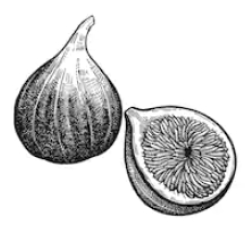
\includegraphics[width=1in,height=1.25in,clip,keepaspectratio]{fig1}}]{Michael Shell}
Use $\backslash${\tt{begin\{IEEEbiography\}}} and then for the 1st argument use $\backslash${\tt{includegraphics}} to declare and link the author photo.
Use the author name as the 3rd argument followed by the biography text.
\end{IEEEbiography}

\vspace{11pt}

\bf{If you will not include a photo:}\vspace{-33pt}
\begin{IEEEbiographynophoto}{John Doe}
Use $\backslash${\tt{begin\{IEEEbiographynophoto\}}} and the author name as the argument followed by the biography text.
\end{IEEEbiographynophoto}




\vfill

\end{document}


